\section{Montáž a opravy BGA a QFN pouzder}
-popis pouzder, technologie montáže a opravy se zaměřením na odlišnosti uvedených jednotlivých pouzder

\subsection{BGA}
Pouzdra BGA(Ball Grid Array) jsou realizována vytvořením souboru pájkových kuliček na spodní straně (základně) pouzdra. Tímto uspořádáním vývodů oproti pouzdrům s vývody na čtyřech (dvou) stranách je možno dosáhnout u stejného rozměru pouzdra většího počtu vývodů, nebo při
stejném počtu vývodů a stejné ploše čipu je rozteč vývodů u pouzder BGA výrazně větší. Kromě vyšší spolehlivosti to přináší i další výhodu - schopnost samovystředění těchto součástek při pájení přetavením.

\subsection{QFN}
QFN - Quad-Flat No-leads. Nevím jak to popsat. Prostě vývody na všech čtyrech stranách, které jsou umístěny přímo na pouzdře-nezabírají místo, dají se pájet poměrně dobře i ručně, největší problém "thermal pad" na spodu QFN-někdy nejde ani za boha všehomoucího odpájet a dřív se zničí součástka.

\subsection{Technologie montáže a opravy se zaměřením na odlišnosti uvedených jednotlivých pouzder}
\subsubsection{Montáž pouzder BGA}
Montáží pouzder BGA rozumíme jejich osazení a zapájení. To lze provést buď osazovacím
automatem přímo na výrobní lince (pájení pak probíhá spolu s ostatními součástkami v
uzavřeném homogenním prostředí pece), nebo ručně pomocí opravárenských stanic. V případě
výrobní linky je celý proces plně automatizován a zásahy obsluhy nejsou vyžadovány. 

Objeví-li se však na výstupu vadné nebo špatně zapájené pouzdro, dá se opravit či vyměnit pouze na opravárenské stanici. Předpokladem dobrého osazení pouzdra BGA je vzájemné sesouhlasení kuličkových vývodů na spodní straně pouzdra s pájecími ploškami na DPS. To lze docílit dvěma způsoby. 

Buď je opticky porovnán obrys pouzdra BGA se servisním potiskem či montážními značkami na DPS (osazuje se takzvaně „na obrys součástky“), nebo jsou pomocí speciální optiky přímo sesouhlaseny jednotlivé vývody s pájecími ploškami. 

Je zřejmé, že druhý způsob je daleko přesnější a pohodlnější, nicméně vzhledem k samovystřeďovací schopnosti pouzder BGA, viz. níže, jsou v praxi použitelné oba způsoby. Jakmile jsou vývody sesouhlasené, provádí se mechanické osazení. Na pájecích ploškách DPS přitom musí být naneseno tavidlo nebo pájecí pasta.

\textbf{Efekt dvojího poklesu} spočívá v postupném klesání pouzdra během pájení.
První pokles nastane v okamžiku přetavení pájecí pasty (je-li použita) nebo při lehkém natavení kuliček v místě obou kontaktních ploch. V případě eutektické slitiny SnPb nastává při 183 $^{\circ}$C a pouzdro při něm klesne asi o 10-20 \% vzdálenosti mezi ním a DPS. Jakmile se kuličky nataví v celém svém objemu, klesnou vlivem hmotnosti pouzdra ještě více - asi o 20-30 \% původní vzdálenosti mezi pouzdrem a DPS. Teprve nyní dojde k dokonalému smočení pájecích ploch (i přes okraje) a ke vzniku difúzních intermetalických vrstev. Vlivem povrchového napětí se také vyhladí povrch spoje a v bezprostřední blízkosti pájecích ploch se vytvoří meniskus ze zbytků tavidla. Druhý pokles obvykle nastává na vrcholu teplotní křivky - asi při 220 $^{\circ}$C (v případě eutektické slitiny SnPb).

\begin{figure}[h]
   \begin{center}
     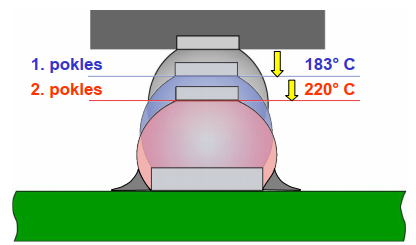
\includegraphics[scale=0.6]{images/Pokles.png}
   \end{center}
   \caption{Dvojí pokles}
\end{figure}

\textbf{Samovystřeďovací schopnost} je jev, kdy dynamické síly povrchového napětí
roztavené pájky způsobí, že v okamžiku druhého poklesu dojde k samovolnému vystředění
pouzdra na pájecích ploškách. Z toho důvodu není nutné pouzdra při osazení naprosto přesně sesadit. Samovystřeďovací schopnost funguje i při 50 \% přesahu vývodu mimo pájecí plošku. Při větší odchylce už hrozí „přeskočení“ pouzdra na vedlejší pájecí plošky.

\begin{figure}[h]
   \begin{center}
     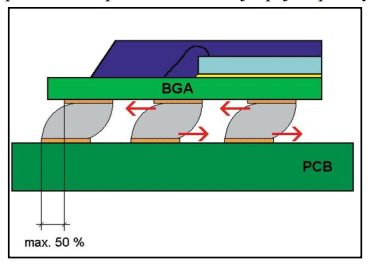
\includegraphics[scale=0.6]{images/Samo.png}
   \end{center}
   \caption{Samovystřeďovací schopnost}
\end{figure}

Při pájení BGA pouzder (stejně jako u ostatních součástek) existuje i nebezpečí zkratů a pájkových můstků mezi vývody pouzdra BGA. Zkraty u BGA pouzder ale nejdou jednoduše
odstranit. Při opravě je nutné celé pouzdro odstranit a připájet nové (nebo původní po provedení reballingu). Tato operace je příliš pracná, a tak je třeba se zkratů co nejvíce vyvarovat.
Zkraty vznikají obvykle z těchto důvodů:
\begin{itemize}
\item špatně natisknutá pájecí pasta, nebo nesprávné množství,
\item nepřesně osazené pouzdro,
\item příliš velká hmotnost pouzdra,
\item nadměrný tlak horkého vzduchu,
\item příliš vysoká pájecí teplota,
\item nadměrné množství nebo nevhodný typ tavidla,
\item prohnutí pouzdra nebo DPS během pájení
\end{itemize}

\subsubsection{Opravy pouzder BGA}
Opravou BGA je myšlen případ, kdy součástka samotná je v pořádku, pouze se ji
nepodařilo správně zapájet, nebo se v důsledku stárnutí některé spoje přerušily. V praxi se sice
takové součástky obvykle rovnou vyměňují, ale v případě, že nové BGA je nedostupné nebo
příliš drahé, je oprava také řešením. V obou dvou případech lze postup shrnout do následujících
kroků:
\begin{itemize}
\item odpájení vadného nebo špatně zapájeného pouzdra,
\item v případě vadné součástky se očistí pájecí plochy na DPS a provede se montáž nového
pouzdra,
\item je-li součástka použitelná, očistí se pájecí plochy na DPS i na součástce,
\item na očištěném pouzdře se provede „reballing“ (obnova kuličkových vývodů),
\item na DPS se nanese tavidlo nebo pájecí pasta (přes speciální minišablonu),
\item pomocí opravárenské stanice se provede montáž nové součástky,
\item provede se kontrola správného zapájení (opticky, rentgenem, elektricky..)
\end{itemize}

























